\documentclass{article}
\usepackage{listings}
\usepackage{jlcode}
\usepackage{graphicx}
\usepackage{layout}
\usepackage{physics}
\usepackage{float}

\title{CAAM 519, Homework $\#2$}
\author{\texttt{ask15}}
\date{September 30, 2022}
\begin{document}
\maketitle
\section*{Section 1: Verifying the correctness of the Forward Euler and explicit midpoint ODE solver (Part 3)}
\subsection*{1}
\begin{figure}[H]
  \centering
  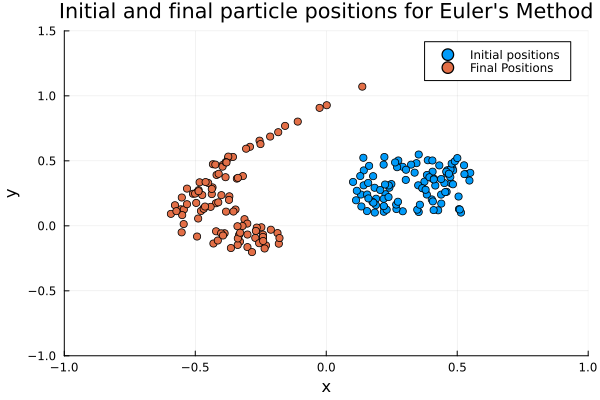
\includegraphics[width=4in]{plot5.png}
\end{figure}

\begin{figure}[H]
  \centering
  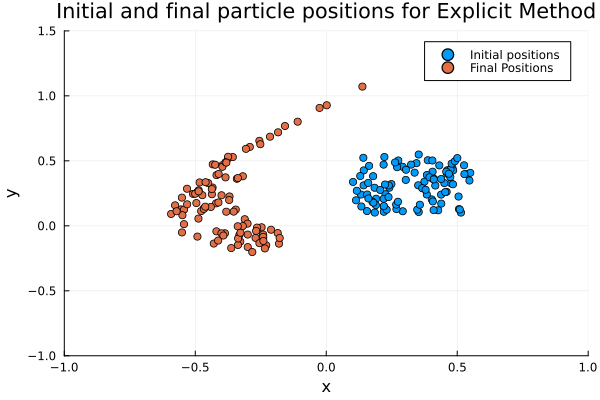
\includegraphics[width=4in]{plot6.png}
\end{figure}
\subsection*{2}
\begin{figure}[H]
  \centering
  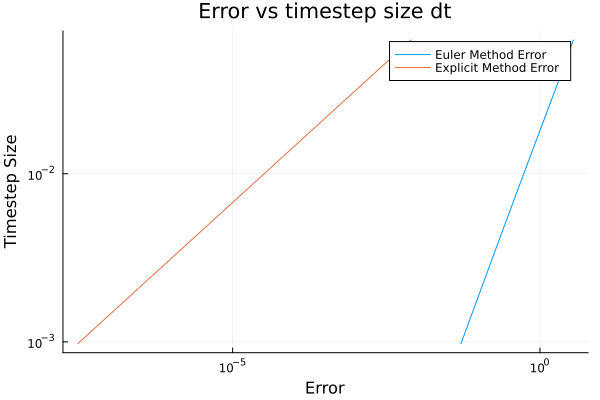
\includegraphics[width=4in]{plot1.png}
\end{figure}

As the timestep size decreases, the error decreases as expected because we are now approximating the derivative at finer time intervals. Thus, as the timestep size decreases, the errors for each method converge to zero.

\section*{Section 2: Analyzing the efficiency of your ``rhs!'' function (Part 2)}
\subsection*{1}
\begin{jllisting}
  MethodInstance for rhs!(::Matrix{Float64}, ::Matrix{Float64}, ::Float64, ::Float64)
  from rhs!(du, u, parameters, t) in Main at c:\Users\Anwar Khaddage\Documents\Julia VS\Juliademo-\part_2.jl:6
  Arguments
  #self#::Core.Const(rhs!)
  du::Matrix{Float64}
  u::Matrix{Float64}
  parameters::Float64
  t::Float64
  Locals
  @_6::Union{Nothing, Tuple{Int64, Int64}}
  num_particles::Int64
  i::Int64
  Body::Nothing
  1 ─       (num_particles = Main.size(u, 2))
  │   %2  = (1:num_particles)::Core.PartialStruct(UnitRange{Int64}, Any[Core.Const(1), Int64])
  │         (@_6 = Base.iterate(%2))
  │   %4  = (@_6 === nothing)::Bool
  │   %5  = Base.not_int(%4)::Bool
  └──       goto #4 if not %5
  2 ┄ %7  = @_6::Tuple{Int64, Int64}
  │         (i = Core.getfield(%7, 1))
  │   %9  = Core.getfield(%7, 2)::Int64
  │   %10 = Base.getindex(u, 1, i)::Float64
  │   %11 = Base.getindex(u, 2, i)::Float64
  │   %12 = Main.v_x(%10, %11, t, parameters)::Float64
  │         Base.setindex!(du, %12, 1, i)
  │   %14 = Base.getindex(u, 1, i)::Float64
  │   %15 = Base.getindex(u, 2, i)::Float64
  │   %16 = Main.v_y(%14, %15, t, parameters)::Float64
  │         Base.setindex!(du, %16, 2, i)
  │         (@_6 = Base.iterate(%2, %9))
  │   %19 = (@_6 === nothing)::Bool
  │   %20 = Base.not_int(%19)::Bool
  └──       goto #4 if not %20
  3 ─       goto #2
  4 ┄       return nothing

\end{jllisting}


\subsection*{2}
\begin{jllisting}
  1.300 ns (0 allocations: 0 bytes)
\end{jllisting}

\section*{Section 3: Analyzing the efficiency of your solver (Part 3)}
\subsection*{1}
\begin{jllisting}

  MethodInstance for (::var''#solve##kw'')(::NamedTuple{(:num_saved_steps,), Tuple{Int64}}, ::typeof(solve), ::ForwardEuler, ::Matrix{Float64}, ::typeof(rhs!), ::Tuple{Int64, Int64}, ::Float64, ::Float64)
  from (::var''#solve##kw'')(::Any, ::typeof(solve), method::ForwardEuler, u0, rhs!, tspan, dt, parameters) in Main at c:\Users\Anwar Khaddage\Documents\Julia VS\Juliademo-\part_1.jl:12
  Arguments
  _::Core.Const(var''#solve##kw''())
  @_2::NamedTuple{(:num_saved_steps,), Tuple{Int64}}
  @_3::Core.Const(solve)
  method::Core.Const(ForwardEuler())
  u0::Matrix{Float64}
  rhs!::Core.Const(rhs!)
  tspan::Tuple{Int64, Int64}
  dt::Float64
  parameters::Float64
  Locals
  num_saved_steps::Int64
  @_11::Int64
  Body::Tuple{Matrix{Float64}, Int64}
  1 ─ %1  = Base.haskey(@_2, :num_saved_steps)::Core.Const(true)
  │         Core.typeassert(%1, Core.Bool)
  │         (@_11 = Base.getindex(@_2, :num_saved_steps))
  └──       goto #3
  2 ─       Core.Const(:(@_11 = 1))
  3 ┄ %6  = @_11::Int64
  │         (num_saved_steps = %6)
  │   %8  = (:num_saved_steps,)::Core.Const((:num_saved_steps,))
  │   %9  = Core.apply_type(Core.NamedTuple, %8)::Core.Const(NamedTuple{(:num_saved_steps,)})
  │   %10 = Base.structdiff(@_2, %9)::Core.Const(NamedTuple())
  │   %11 = Base.pairs(%10)::Core.Const(Base.Pairs{Symbol, Union{}, Tuple{}, NamedTuple{(), Tuple{}}}())
  │   %12 = Base.isempty(%11)::Core.Const(true)
  │         Core.typeassert(%12, Core.Bool)
  └──       goto #5
  4 ─       Core.Const(:(Base.kwerr(@_2, @_3, method, u0, rhs!, tspan, dt, parameters)))
  5 ┄ %16 = Main.:(var"#solve#6")(num_saved_steps, @_3, method, u0, rhs!, tspan, dt, parameters)::Tuple{Matrix{Float64}, Int64}
  └──       return %16
\end{jllisting}
\\
\begin{jllisting}
  MethodInstance for (::var''#solve##kw'')(::NamedTuple{(:num_saved_steps,), Tuple{Int64}}, ::typeof(solve), ::ExplicitMidpoint{Matrix{Float64}}, ::Matrix{Float64}, ::typeof(rhs!), ::Tuple{Int64, Int64}, ::Float64, ::Float64)
  from (::var''#solve##kw'')(::Any, ::typeof(solve), method::ExplicitMidpoint, u0, rhs!, tspan, dt, parameters) in Main at c:\Users\Anwar Khaddage\Documents\Julia VS\Juliademo-\part_1.jl:47
  Arguments
  _::Core.Const(var''#solve##kw''())
  @_2::NamedTuple{(:num_saved_steps,), Tuple{Int64}}
  @_3::Core.Const(solve)
  method::ExplicitMidpoint{Matrix{Float64}}
  u0::Matrix{Float64}
  rhs!::Core.Const(rhs!)
  tspan::Tuple{Int64, Int64}
  dt::Float64
  parameters::Float64
  Locals
  num_saved_steps::Int64
  │         (@_11 = Base.getindex(@_2, :num_saved_steps))
  └──       goto #3
  2 ─       Core.Const(:(@_11 = 1))
  3 ┄ %6  = @_11::Int64
  │         (num_saved_steps = %6)
  │   %8  = (:num_saved_steps,)::Core.Const((:num_saved_steps,))
  │   %9  = Core.apply_type(Core.NamedTuple, %8)::Core.Const(NamedTuple{(:num_saved_steps,)})
  │   %10 = Base.structdiff(@_2, %9)::Core.Const(NamedTuple())
  │   %11 = Base.pairs(%10)::Core.Const(Base.Pairs{Symbol, Union{}, Tuple{}, NamedTuple{(), Tuple{}}}())                                                                          )})
  │   %12 = Base.isempty(%11)::Core.Const(true)
  │         Core.typeassert(%12, Core.Bool)                                               , Tuple{}}}())
  └──       goto #5
  4 ─       Core.Const(:(Base.kwerr(@_2, @_3, method, u0, rhs!, tspan, dt, parameters)))
  5 ┄ %16 = Main.:(var"#solve#7")(num_saved_steps, @_3, method, u0, rhs!, tspan, dt, parameters)::Tuple{Matrix{Float64}, Int64}
  └──       return %16
\end{jllisting}

\subsection*{2}
\begin{figure}[H]
  \centering
  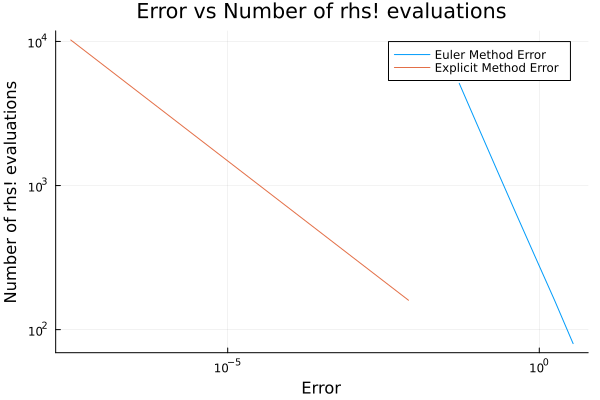
\includegraphics[width=4in]{plot2.png}
\end{figure}
\end{document}
